\graphicspath{{../Graphics/Cpt1-Charactz/}}

	\begin{figure}[H]
		\centering
		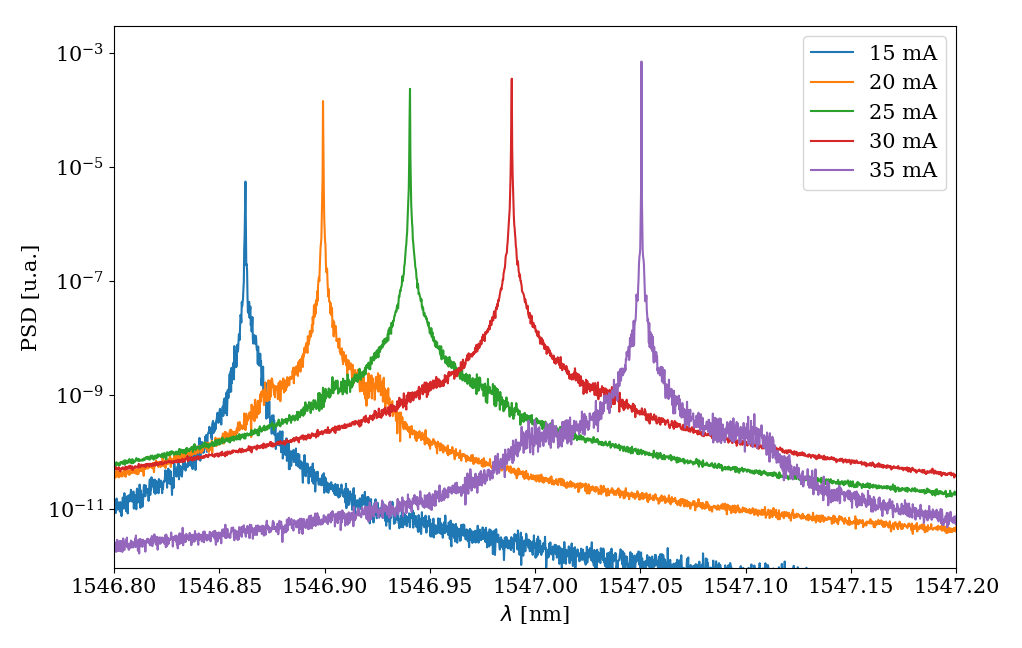
\includegraphics[scale=0.5]{Espectros.png}
		\caption{\label{Img:widgets}el pie de pagina que le quieras 	poner a la imagen}
	\end{figure}

	\begin{table}[H]
		\centering
		\begin{tabular}{c c}
			\hline
			$I_{Bias}$ & $\lambda$ \\\hline 
			15 & 1546.86 \\
			20 & 1546.90 \\
			25 & 1546.94 \\
			30 & 1546.99 \\
			35 & 1547.05 \\\hline
		\end{tabular}
		\caption{\label{tab:label}caption}
	
	\end{table}

	\begin{figure}[H]
		\centering
		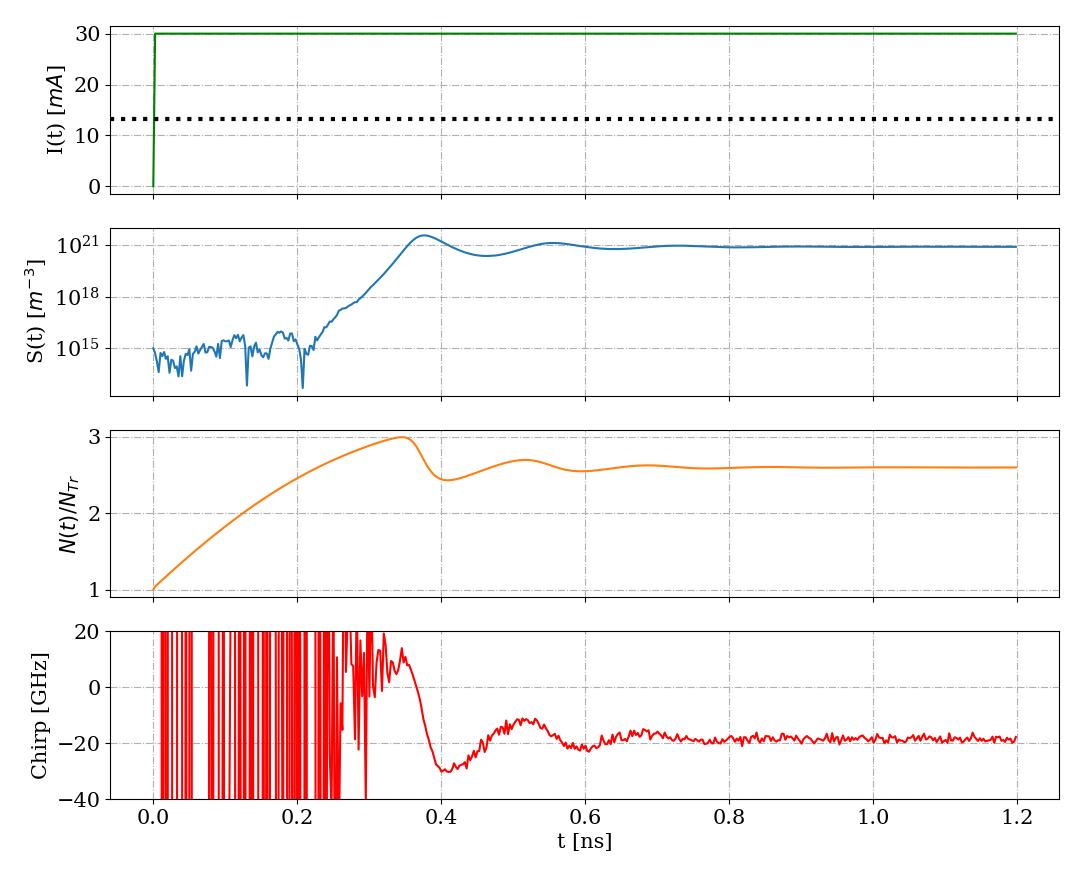
\includegraphics[scale=0.5]{transitorio.png}
		\caption{\label{fig:transitorio}Transitorio}	
	\end{figure}

		\begin{figure}[H]
			\centering
			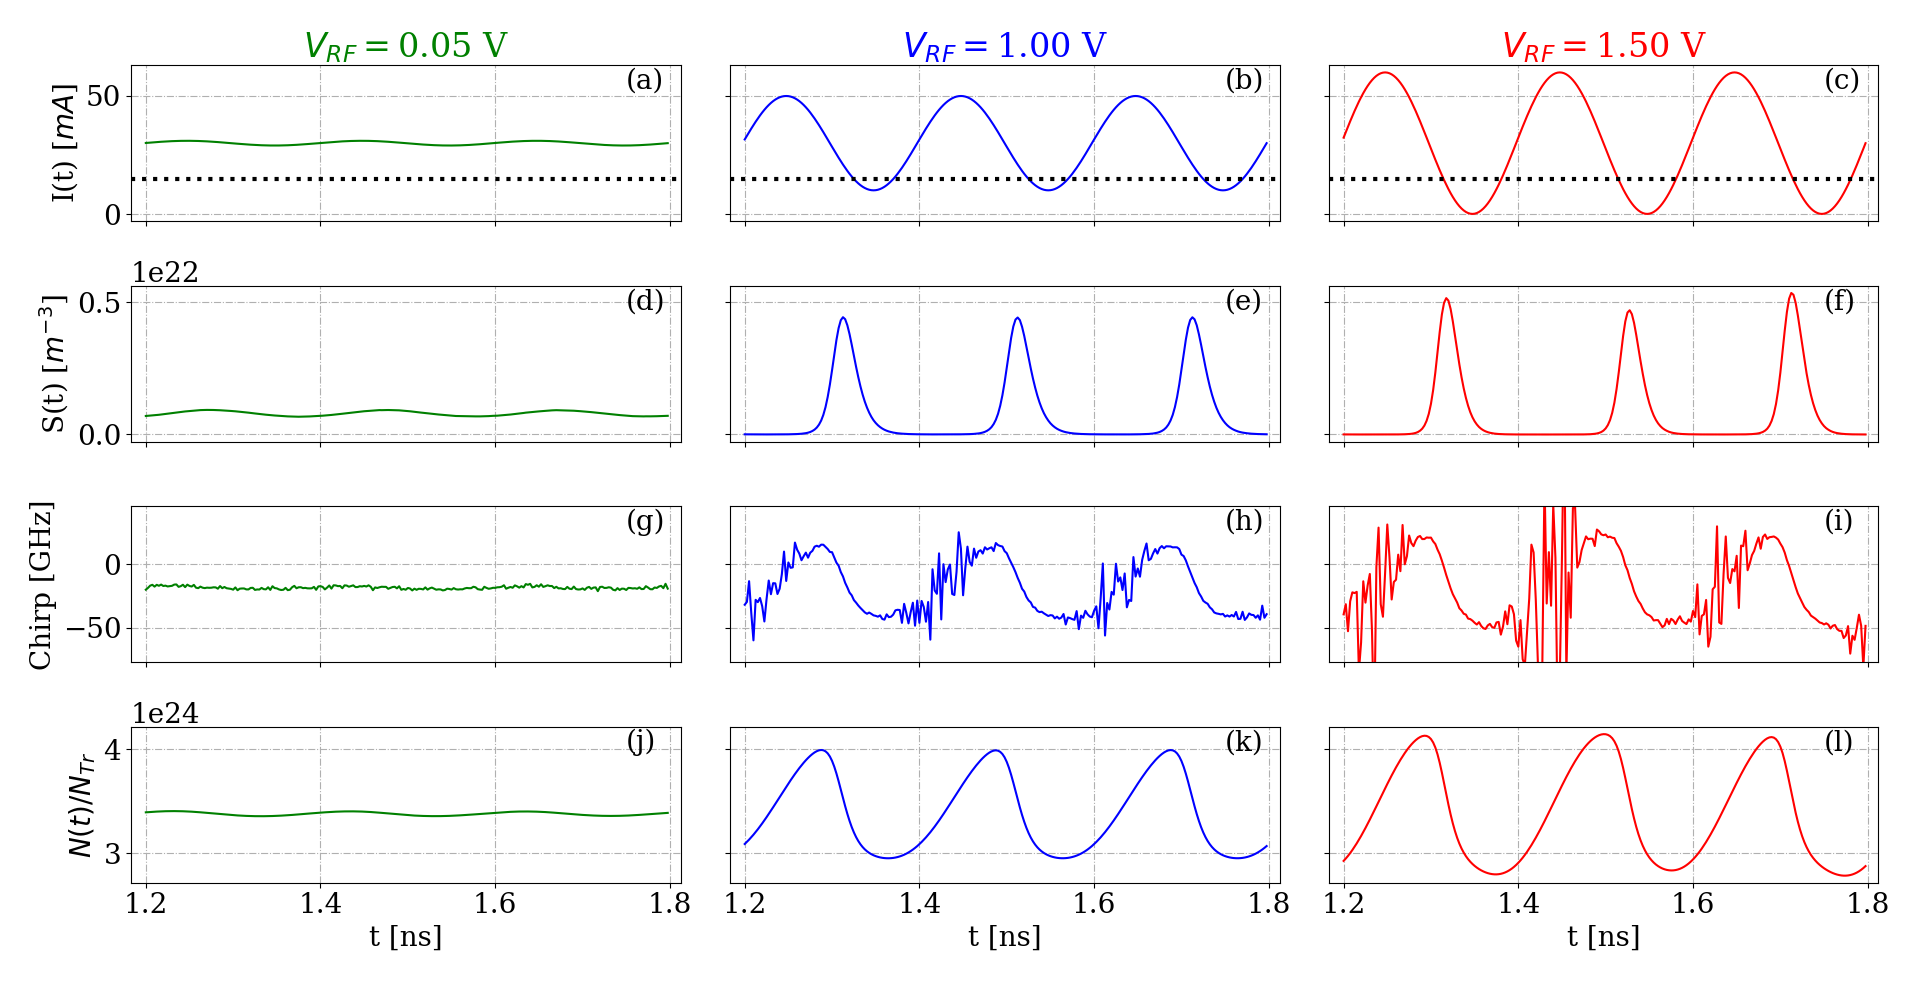
\includegraphics[width=1.0\linewidth]{rateEquations.png}
			\caption{\label{fig:rateEquations}RateEquations}	
		\end{figure}

		\begin{figure}[H]
			\centering
			\includegraphics[width=1.0\linewidth]{hola.png}
			\caption{\label{fig:rateEquations}RateEquations}	
		\end{figure}
